\subsubsection{Model}


\class{Sensorthing}
public abstract class Sensorthing<SensorthingT extends Sensorthing<SensorthingT>>
\\\\
\begin{minipage}{0.3\textwidth}
	\begin{figure}[H]
		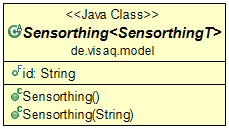
\includegraphics[scale = 0.5
		]{media/frontend/model/SensorthingClass.png}
	\end{figure}
\end{minipage} \hfill
\begin{minipage}{0.6\textwidth}
	Die abstrakte Klasse Sensorthing kapselt den Inhalt der Klasse Sensorthing des Backends. Sie wird von allen Sensorthing Klassen des Frontend implementiert.
\end{minipage}

Attribute:
\begin{itemize}
	\item \emph{public final String id} Die eindeutige Identifikation des Sensorthing Objekts.
\end{itemize}
Methoden:
\begin{itemize}
	\item \emph{public Sensorthing()} Konstruktor der Klasse Sensorthing, setzt die ID auf null.
	\item \emph{public Sensorthing(String id)} Konstruktor der Klasse Sensorthing, speichert die übergebene ID.
\end{itemize}

\rule{\textwidth}{0.4pt}
\class{SensorthingTimeStamp}
public interface SensorthingsTimeStamp
\\\\
\begin{minipage}{0.3\textwidth}
	\begin{figure}[H]
		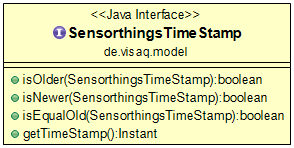
\includegraphics[scale = 0.5
		]{media/frontend/model/SensorthingTimeStampClass.png}
	\end{figure}
\end{minipage} \hfill
\begin{minipage}{0.6\textwidth}
	Das Interface SensorthingTimeStamp im Frontend entspricht genau dem Interface SensorthingTimeStamp im Backend. Es enthält die Methoden für alle Sensorthing Klassen mit Zeitstempel.
\end{minipage}

Methoden:
\begin{itemize}
	\item \emph{public boolean isOlder(SensorthingTimeStamp other)} Vergleicht ob ein übergebener Zeitstempel älter ist als der Zeitstempel des Objekts, Rückgabewert ist eine boolsche Variable.
	\item \emph{public boolean isNewer(SensorthingTimeStamp other)} Vergleicht ob ein übergebener Zeitstempel neuer ist als der Zeitstempel des Objekts, Rückgabewert ist eine boolsche Variable.
	\item \emph{public boolean isEqualOld(SensorthingTimeStamp other)} Vergleicht ob ein übergebener Zeitstempel gleich alt ist wie der Zeitstempel des Objekts, Rückgabewert ist eine boolsche Variable.
	\item \emph{public Instant getTimeStamp()} Gibt den Zeitstempel des Objekts zurück.
\end{itemize}

\rule{\textwidth}{0.4pt}
\class{Datastream}
public class Datastream extends Sensorthing<Datastream>
\\\\
\begin{minipage}{0.3\textwidth}
	\begin{figure}[H]
		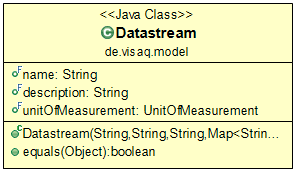
\includegraphics[scale = 0.5
		]{media/frontend/model/DatastreamClass.png}
	\end{figure}
\end{minipage} \hfill
\begin{minipage}{0.6\textwidth}
	\modelFrontendDescription{Datastream}
\end{minipage}

Attribute:
\begin{itemize}
	\item \emph{public final String name} Der Name des Datastreams
	\item \emph{public final String description} Die Beschreibung des Datastreams
	\item \emph{public final UnitOfMeasurement unitOfMeasurement} Die Maßeinheit
\end{itemize}
Methoden:
\begin{itemize}
	\item \emph{public Datastream(String id, String name, String description, Map<String, Object> properties, UnitOfMeasurement unitOfMeasurement))} \constructorDescription{Datastream}
	\item \emph{public boolean equals(Object obj)} \equalsDescription{Datastream}
\end{itemize}

\rule{\textwidth}{0.4pt}
\class{FeatureOfInterest}
public class FeatureOfInterest extends Sensorthing<FeatureOfInterest>
\\\\
\begin{minipage}{0.3\textwidth}
	\begin{figure}[H]
		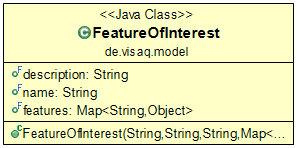
\includegraphics[scale = 0.5
		]{media/frontend/model/FeatureOfInterestClass.png}
	\end{figure}
\end{minipage} \hfill
\begin{minipage}{0.6\textwidth}
	\modelFrontendDescription{FeatureOfInterest}
\end{minipage}

Attribute:
\begin{itemize}
	\item \emph{public final String name} Der Name des FeatureOfInterest
	\item \emph{public final String description} Die Beschreibung des FeatureOfInterest
	\item \emph{public final Map<String, Object> features} Merkmale(Features)
\end{itemize}
Methoden:
\begin{itemize}
	\item \emph{public FeatureOfInterest(String id, String description, String name, Map<String, Object> features)} \constructorDescription{FeatureOfInterest}
	\item \emph{public boolean equals(Object obj)} \equalsDescription{FeatureOfInterest}
\end{itemize}

\rule{\textwidth}{0.4pt}
\class{HistoricalLocation}
public class HistoricalLocation extends Sensorthing<Datastream> implements SensorthingsTimeStamp
\\\\
\begin{minipage}{0.3\textwidth}
	\begin{figure}[H]
		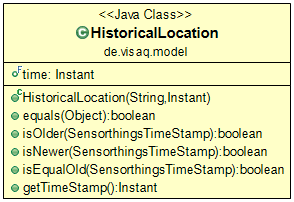
\includegraphics[scale = 0.5
		]{media/frontend/model/HistoricalLocationClass.png}
	\end{figure}
\end{minipage} \hfill
\begin{minipage}{0.6\textwidth}
	\modelFrontendDescription{HistoricalLocation} Zudem implementiert HistoricalLocation das Interface SensorthingTimeStamp.
\end{minipage}

Attribute:
\begin{itemize}
	\item \emph{public final Instant time} Der Zeitpunkt
\end{itemize}
Methoden:
\begin{itemize}
	\item \emph{public HistoricalLocation(String id, Instant time)} \constructorDescription{HistoricalLocation}
	\item \emph{public boolean equals(Object obj)} \equalsDescription{HistoricalLocation}
	\item \emph{public boolean isOlder(SensorthingTimeStamp other)} Vergleicht ob ein übergebener Zeitstempel älter ist als der Zeitstempel des HistoricalLocation Objekts, Rückgabewert ist eine boolsche Variable.
	\item \emph{public boolean isNewer(SensorthingTimeStamp other)} Vergleicht ob ein übergebener Zeitstempel neuer ist als der Zeitstempel des HistoricalLocation Objekts, Rückgabewert ist eine boolsche Variable.
	\item \emph{public boolean isEqualOld(SensorthingTimeStamp other)} Vergleicht ob ein übergebener Zeitstempel gleich alt ist wie der Zeitstempel des HistoricalLocation Objekts, Rückgabewert ist eine boolsche Variable.
	\item \emph{public Instant getTimeStamp()} Gibt den Zeitstempel des HistoricalLocation Objekts zurück.
\end{itemize}

\rule{\textwidth}{0.4pt}
\class{Location}
public class Location extends Sensorthing<Location>
\\\\
\begin{minipage}{0.3\textwidth}
	\begin{figure}[H]
		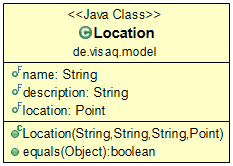
\includegraphics[scale = 0.5
		]{media/frontend/model/LocationClass.png}
	\end{figure}
\end{minipage} \hfill
\begin{minipage}{0.6\textwidth}
	\modelFrontendDescription{Location}
\end{minipage}

Attribute:
\begin{itemize}
	\item \emph{public final String name} Der Name der Location
	\item \emph{public final String description} Die Beschreibung der Location
	\item \emph{public final Point location} Die Koordinaten des Orts
\end{itemize}
Methoden:
\begin{itemize}
	\item \emph{public Location(String id, String name, String description, Point location)} \constructorDescription{Location}
	\item \emph{public boolean equals(Object obj)} \equalsDescription{Location}
\end{itemize}
\clearpage %opt
\rule{\textwidth}{0.4pt}
\class{Observation}
public class Observation extends Sensorthing<FeatureOfInterest> implements SensorthingsTimeStamp
\\\\
\begin{minipage}{0.3\textwidth}
	\begin{figure}[H]
		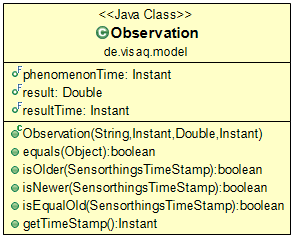
\includegraphics[scale = 0.5
		]{media/frontend/model/ObservationClass.png}
	\end{figure}
\end{minipage} \hfill
\begin{minipage}{0.6\textwidth}
	\modelFrontendDescription{Observation} Zudem implementiert Observation das Interface SensorthingTimeStamp.
\end{minipage}

Attribute:
\begin{itemize}
	\item \emph{public final Instant phenomenonTime} Der Zeitpunkt der Observation
	\item \emph{public final Double result} Die Beschreibung der Observation
	\item \emph{public final Instant resultTime} Der Zeitpunkt des gemessenen Resultats.
\end{itemize}
Methoden:
\begin{itemize}
	\item \emph{public Observation(String id, Instant phenomenonTime, Double result, Instant resultTime)} \constructorDescription{Observation}
	\item \emph{public boolean equals(Object obj)} \equalsDescription{Observation}
	\item \emph{public boolean isOlder(SensorthingTimeStamp other)} Vergleicht ob ein übergebener Zeitstempel älter ist als der Zeitstempel des Observation Objekts, Rückgabewert ist eine boolsche Variable.
	\item \emph{public boolean isNewer(SensorthingTimeStamp other)} Vergleicht ob ein übergebener Zeitstempel neuer ist als der Zeitstempel des Observation Objekts, Rückgabewert ist eine boolsche Variable.
	\item \emph{public boolean isEqualOld(SensorthingTimeStamp other)} Vergleicht ob ein übergebener Zeitstempel gleich alt ist wie der Zeitstempel des Observation Objekts, Rückgabewert ist eine boolsche Variable.
	\item \emph{public Instant getTimeStamp()} Gibt den Zeitstempel des Observation Objekts zurück.
\end{itemize}

\rule{\textwidth}{0.4pt}
\class{ObservedProperty}
public class ObservedProperty extends Sensorthing<ObservedProperty>
\\\\
\begin{minipage}{0.3\textwidth}
	\begin{figure}[H]
		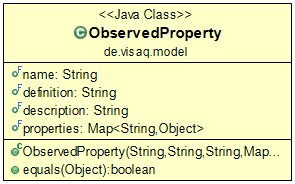
\includegraphics[scale = 0.5
		]{media/frontend/model/ObservedPropertyClass.png}
	\end{figure}
\end{minipage} \hfill
\begin{minipage}{0.6\textwidth}
	\modelFrontendDescription{ObservedProperty}
\end{minipage}

Attribute:
\begin{itemize}
	\item \emph{public final String name} Der Name der ObservedProperty
	\item \emph{public final String definition} Die Definition der ObservedProperty
	\item \emph{public final String description} Die Beschreibung der ObservedProperty
	\item \emph{public final Map<String, Object> properties} Die Eigenschaften der ObservedProperty
\end{itemize}
Methoden:
\begin{itemize}
	\item \emph{public Location(String id, String name, String description, Point location)} \constructorDescription{ObservedProperty}
	\item \emph{public boolean equals(Object obj)} \equalsDescription{ObservedProperty}
\end{itemize}

\rule{\textwidth}{0.4pt}
\class{Sensor}
public class Sensor extends Sensorthing<Sensor>
\\\\
\begin{minipage}{0.3\textwidth}
	\begin{figure}[H]
		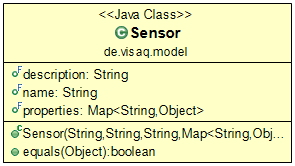
\includegraphics[scale = 0.5
		]{media/frontend/model/SensorClass.png}
	\end{figure}
\end{minipage} \hfill
\begin{minipage}{0.6\textwidth}
	\modelFrontendDescription{Sensor}
\end{minipage}

Attribute:
\begin{itemize}
	\item \emph{public final String name} Der Name des Sensors
	\item \emph{public final String description} Die Beschreibung des Sensors
	\item \emph{public final Map<String, Object> properties} Die Eigenschaften des Sensors
\end{itemize}
Methoden:
\begin{itemize}
	\item \emph{Sensor(String id, String description, String name, Map<String, Object> properties)} \constructorDescription{Sensor}
	\item \emph{public boolean equals(Object obj)} \equalsDescription{Sensor}
\end{itemize}
\clearpage %opt
\rule{\textwidth}{0.4pt}
\class{Thing}
public class Thing extends Sensorthing<Thing>
\\\\
\begin{minipage}{0.3\textwidth}
	\begin{figure}[H]
		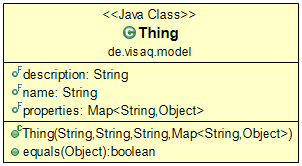
\includegraphics[scale = 0.5
		]{media/frontend/model/ThingClass.png}
	\end{figure}
\end{minipage} \hfill
\begin{minipage}{0.6\textwidth}
	\modelFrontendDescription{Thing}
\end{minipage}

Attribute:
\begin{itemize}
	\item \emph{public final String name} Der Name des Thing
	\item \emph{public final String description} Die Beschreibung des Thing
	\item \emph{public final Map<String, Object> properties} Die Eigenschaften des Thing
\end{itemize}
Methoden:
\begin{itemize}
	\item \emph{Sensor(String id, String description, String name, Map<String, Object> properties)} \constructorDescription{Thing}
	\item \emph{public boolean equals(Object obj)} \equalsDescription{Thing}
\end{itemize}
\clearpage %opt
\rule{\textwidth}{0.4pt}
\class{UnitOfMeasurement}
public class UnitOfMeasurement
\\\\
\begin{minipage}{0.3\textwidth}
	\begin{figure}[H]
		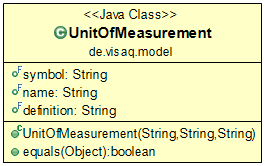
\includegraphics[scale = 0.5
		]{media/frontend/model/UnitOfMeasurementClass.png}
	\end{figure}
\end{minipage} \hfill
\begin{minipage}{0.6\textwidth}
	\modelFrontendDescription{UnitOfMeasurement} UnitOfMeasurement beschreibt die Einheit in der Daten repräsentiert werden.
\end{minipage}

Attribute:
\begin{itemize}
	\item \emph{public final String name} Der Name der UnitOfMeasurement
	\item \emph{public final String description} Die Beschreibung der UnitOfMeasurement
	\item \emph{public final Map<String, Object> properties} Die Eigenschaften der UnitOfMeasurement
\end{itemize}
Methoden:
\begin{itemize}
	\item \emph{Sensor(String id, String description, String name, Map<String, Object> properties)} \constructorDescription{UnitOfMeasurement}
	\item \emph{public boolean equals(Object obj)} \equalsDescription{UnitOfMeasurement}
\end{itemize}
\clearpage %opt
\rule{\textwidth}{0.4pt}
\class{SensorDatum}
public class SensorDatum
\\\\
\begin{minipage}{0.3\textwidth}
	\begin{figure}[H]
		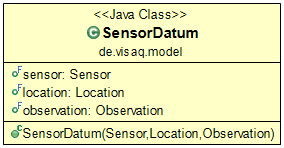
\includegraphics[scale = 0.5
		]{media/frontend/model/SensorDatumClass.png}
	\end{figure}
\end{minipage} \hfill
\begin{minipage}{0.6\textwidth}
	Die Klasse SensorDatum kapselt die Daten von einem Sensor, seiner Postion und eine Observation. Die Klasse wird zur Datenaufbereitung genutzt.
\end{minipage}

Attribute:
\begin{itemize}
	\item \emph{public final Sensor sensor} Der Sensor
	\item \emph{public final Location location} Die Position des Sensors
	\item \emph{public final Observation observation} Die gemessenen Daten des Sensors
\end{itemize}
Methoden:
\begin{itemize}
	\item \emph{Sensor(String id, String description, String name, Map<String, Object> properties)} \constructorDescription{SensorDatum}
\end{itemize}
